\documentclass[preprint,a4paper, 10pt, 5p]{elsarticle}
% preprint , review, 1p, 3p, 5p

\usepackage[utf8]{inputenc}
\usepackage[T1]{fontenc}
\usepackage{lineno,hyperref}
\modulolinenumbers[5]
\usepackage{amsmath,amssymb,amsfonts}
\usepackage{algorithm}
\usepackage{algorithmic}
\usepackage{graphicx}
\usepackage{textcomp}
\usepackage{mathtools}
\usepackage{adjustbox}
\usepackage{tabularx}
\usepackage{booktabs}
\usepackage{multirow}
\usepackage{float}
\journal{Journal of xxxxx}

\usepackage[labelfont=bf,justification=raggedright,singlelinecheck=false]{caption}
\captionsetup[figure]{name=Fig. ,labelsep=period}
\captionsetup[table]{labelsep=newline,font=footnotesize}

\renewcommand{\topfraction}{0.9}
\renewcommand{\bottomfraction}{0.8}
\renewcommand{\textfraction}{0.07}
\renewcommand{\floatpagefraction}{0.8}
\renewcommand{\dbltopfraction}{0.9}
\renewcommand{\dblfloatpagefraction}{0.8}
\setcounter{topnumber}{3}
\setcounter{bottomnumber}{2}
\setcounter{totalnumber}{4}
\setcounter{dbltopnumber}{3}
\emergencystretch=1.5em
%% `Elsevier LaTeX' style
\bibliographystyle{elsarticle-num}
%%%%%%%%%%%%%%%%%%%%%%%

\begin{document}

\begin{frontmatter}

\title{Modality Fairness via OGR-Driven Gradient Harmonization: Dynamic Loss Balancing Against Gradient Starvation}

\author[1]{Lakshya}

\author[1]{Amit Kumar Bairwa\corref{cor1}}
\ead{amitkumar.bairwa@jaipur.manipal.edu}

\author[1]{Varun Tiwari\corref{cor1}}
\ead{varun.tiwari@jaipur.manipal.edu}

\address[1]{Department of Artificial Intelligence and Machine Learning, School of Computer Science and Engineering, Manipal University Jaipur, Jaipur--Ajmer Express Highway, Jaipur, India}
\cortext[cor1]{Corresponding authors}

\begin{abstract}
Multi modal learning systems are likely to be stuck in one of such traps and it is known as the Modality Laziness trap whereby they over-respond to the best signal in most instances which happens to be the best signal. Visual signal and ignore the weak signals such as the Audio or Text signal. The unified models are their possible limited by this optimization bias. Although fixes such as Gradient Blending or OGM-GE currently exist with most of them being based on expensive pre-computations or noisy and unstable noise. Insertion which is incapable of following the dynamics of training. In this paper, the Modality is presented. Fairness Controller (MFC), a simple and easy to use solution. The idea behind the MFC is to look at the Overfitting-to-Generalization Ratio (OGR) of each modality and dynamically vary the level to which each modality affects the learning process. We were able to test on a controlled synthetic benchmark, and a real-world CREMA-D emotion recognition (7,442 mel spectrogram samples, 6 classes). MFC-A also reduces the difference in modality imbalance by 38.4\% at synthetic benchmark and it also enhances the gap. robustness by $+4.7\%$ at $\sigma{=}0.5$ and $+2.3\%$ at $\sigma{=}1.0$ noise. At actual CREMA-D data the MFC-A is as well as accurate as at the baseline and diminishes the OGR dispersion by 38.9 percent without incurring any overhead of noise injection.At 1024-dim model capacity, MFC-A yields a +3.1\% accuracy gain over the baseline, confirming its value grows with model size.
\end{abstract}

\begin{keyword}
Multi-modal Learning \sep Modality Laziness \sep Gradient Starvation \sep Loss Balancing \sep Overfitting-to-Generalization Ratio (OGR) \sep Emotion Recognition \sep Dynamic Modulation \sep Modality Fairness Controller (MFC)
\end{keyword}

\end{frontmatter}

\section{Introduction}
The world is tasted in the colourful mixture of impressions. This is what ideally Proposed AI models should do. Nevertheless, such multimodal architectures are usually difficult to train, and powerful ones like Unified Transformers \cite{zhang2023meta}, Image Bind \cite{girdhar2023imagebind}, CLIP \cite{radford2021learning} and Flamingo \cite{alayrac2022flamingo} these become lazy. When one of the modalities (say an image) is easier to learn than the other (say audio) then the model neglects the more difficult task. This will be called a Modality Laziness or Gradient Starvation \cite{pezeshki2021gradient}. The visual features too are generally means puny and arranged; this presents a simple access point leading to the optimizer. Noisey audio or text may be less or excessive. This means that the high visual gradients would tend to absorb the common weights in the model at almost full costs and the other modalities are under-developed. In the real world such as an autonomous car that may have to hear a siren that it cannot see this blindness can be hazardous. Although the various fixes have been enumerated in various recent surveys, like the Balance Benchmark \cite{xu2025balancebenchmark}, most of them are burdensome. Others must be taught a high number of models to get appropriate weights or simply strive to resolve the problem by introducing random noise, again a common hit-or-miss method, like OGM-GE \cite{peng2022balanced}. We propose a more idealistic one the Modality Fairness Controller (MFC). Instead of simply slowing down the fast learner, we pose a simple question: Is this modality in fact generalizing or is it simply memorizing? We can take the first step to having each modality pull its own weight with respect to the actual unified representation by taking the cue of limiting Proposed learning rates by the Generalization Gap.

The visual features are also generally small and arranged and this provides a simple pathway to the optimizer \cite{pezeshki2021gradient}. Well-conditioned loss surface Vision features dense, spatially coherent, low-noise (e.g. CIFAR-10 \cite{krizhevsky2009learning}) features. Audio characteristics, such as speaker-varying, temporally noisy (e.g., CREMA-D \cite{cao2014crema}) create a more rugged and high-variance landscape. Thus, the powerful visual gradients are inclined to attract the shared weights in the model almost entirely and the remaining modalities are under-developed. The implications cannot be seen in normal assessment but are disastrous when stressed modality. The baseline performance of 83.3\% accuracy falls to 48.2\% accuracy with the addition of Gaussian noise (at 1.0) to visual input (a 35-point drop) because the audio encoder was never developed. In autonomous driving, fog or glare produces the same failure. In medical imaging, corrupted scans leave the model unable to fall back on clinical text it never learned.

\subsection*{Root Cause}
The visual features are also normally compact and organized, which offers an easy route to the optimizer \cite{pezeshki2021gradient}. Vision features---dense, spatially coherent, low-noise (e.g., CIFAR-10 \cite{krizhevsky2009learning})---produce a well-conditioned loss surface. Audio features---speaker-dependent, temporally noisy (e.g., CREMA-D \cite{cao2014crema})---produce a rougher, high-variance landscape. Consequently, the strong visual gradients tend to pull the shared weights in the model nearly completely and the rest of the modalities become under-developed.

The consequences are invisible during standard evaluation but severe under modality stress. Proposed experiments show the baseline collapses from 83.3\% to 48.2\% accuracy when Gaussian noise ($\sigma = 1.0$) is added to visual input---a 35-point drop---because the audio encoder was never developed. In the real world such as an autonomous car that may have to hear a siren that it cannot see this blindness can be hazardous.

\subsection*{Limits of Existing Approaches}
While Although recent surveys such as Balance Benchmark \cite{xu2025balancebenchmark} have listed different fixes, most of them are cumbersome. Gradient Blending \cite{wang2020makes} trains $M{+}1$ separate models to compute static blending weights---mathematically principled, but $M{+}2\times$ the compute budget and unable to adapt as training dynamics shift. OGM-GE \cite{peng2022balanced} injects Gaussian noise into the over-performing modality's backward pass---adaptive, but the noise variance $\sigma$ must be hand-tuned and, as Proposed CREMA-D results confirm, over-correction costs $-3.1\%$ accuracy. UWGA \cite{kendall2018multi} weights by uncertainty---but overfit modalities are precisely the high-confidence ones, so it systematically boosts the wrong modality. All these methods share a deeper flaw: they monitor how fast each modality is changing, not whether that change generalizes. A large gradient norm can indicate productive learning or rapid memorization---gradient norms cannot distinguish the two.

\subsection*{Proposed Approach}
We propose the Modality Fairness Controller (MFC-A), built on a novel per-modality metric: the Overfitting-to-Generalization Ratio (OGR).

\begin{equation}
    OGR_m(t) = \frac{\mathcal{L}^{val}_m(t)}{\mathcal{L}^{train}_m(t) + \epsilon}
\end{equation}

When $OGR \approx 1$, a modality is generalizing. When $OGR \gg 1$, it is overfitting. Unlike raw generalization gaps, OGR is scale-invariant and directly comparable across modalities with very different loss magnitudes. The MFC-A monitors per-modality OGRs via an exponential moving average and adjusts each modality's loss weight $\lambda_m$: throttle when $OGR > \tau_{hi}$, amplify when underfitting.
Proposed best variant, MFC-A, uses inverse-OGR weighting with no threshold parameters:
\begin{equation}
      \lambda_m(t) = \frac{2 \cdot \frac{1}{OGR_m(t)}}{\frac{1}{OGR_v(t)} + \frac{1}{OGR_a(t)}}
  \end{equation}
No auxiliary networks, noise injection, or offline pre-computation are needed---overhead is $O(M \cdot H)$ scalars per epoch.

\subsection*{Contributions}
OGR metric: a scale-invariant, gradient-free per-modality generalization diagnostic computed from standard train/val logs.

MFC-A: a closed-loop dynamic loss re-weighting controller operating in a single training run at negligible cost.

Validation on synthetic CIFAR-10/CREMA-D benchmarks and real CREMA-D emotion recognition: 38.4\% OGR gap reduction, best Rob@0.5 (72.9\%) and Rob@1.0 (50.5\%) across all methods---at zero additional FLOPs.

Scaling analysis: MFC gains grow with model capacity ($+0.7\%$ at 128-dim to $+3.1\%$ at 1024-dim), making it most valuable in the large-model regime.

\section{Related Work}

\subsection{Static Re-weighting Strategies}
Multimodal learning has been documented on the imbalance problem. The first to propose the calculation of optimal weights off-line was Gradient Blending \cite{wang2020makes}. They construct the weighting scheme in which unimodal and multimodal baselines are trained to converge to minimize the overfitting gap. Nevertheless, it is computationally prohibitive with large models, and scales in direct proportion to the number of combinations of modality. Other methods that are static such as UWGA (Uncertainty-Weighted Gradient Aggregation) \cite{kendall2018multi} are trying to make use of task uncertainty, although they tend to fail when a single modality is inherently less noisy yet less informative (such as a black screen with perfect silence). Methods inspired by Focal Loss \cite{lin2017focal} have also been implemented but they do not deal with modality imbalance, but deal with class imbalance.

\subsection{Dynamic Modulation Techniques}
Dynamic methods seek to change weights dynamically. OGM-GE \cite{peng2022balanced} keeps a check on the size of gradient updates. When the gradient norm of one modality is changing too rapidly (which means that the modality is converging too fast), OGM-GE adds Gaussian noise to the backward pass of that modality. Although effective, this is based on auxiliary noise generators that may destabilize training and has hyperparameter sensitivity with respect to the noise variance.

\textbf{GradNorm} \cite{chen2018gradnorm} was an early gradient-based approach that normalizes per-task gradient magnitudes to a shared target, preventing any single task from monopolizing the optimizer. \textbf{PCGrad} \cite{yu2020gradient} detects conflicting gradients across tasks and projects them onto each other's normal planes to reduce interference. \textbf{AGM} \cite{li2023boosting} extends this idea to multimodal settings with per-modality adaptive gradient scaling calibrated against a reference modality. \textbf{Multi-loss gradient modulation} \cite{kontras2024improving} jointly modulates multiple loss terms to keep modality-specific gradient magnitudes in balance throughout training. \textbf{OLM} \cite{zong2024balancing} proposes online logit modulation to equalize modal contributions at the prediction level rather than the gradient level. \textbf{MMPareto} \cite{wei2024mmpareto} frames multimodal optimization as a Pareto problem, using unimodal assistance signals to prevent the joint loss surface from collapsing onto the dominant modality. \textbf{AMSA} \cite{wang2023amsa} demonstrates adaptive loss modulation in the sentiment analysis domain. PMR (Progressive Modality Reinforcement) \cite{xu2025balancebenchmark}, employs a momentum-based tracker to rampage the learning rate of the dominant modality. The alignment is modeled in MBPO \cite{liu2025modality} as a preference maximization problem which employs the reinforcement learning to punish hallucinations which are modality specific. We are different in the sense that we offer a closed-loop, parameter-free controller that is expressly on the basis of the Generalization Gap, which does not require the complexity of RL or is unstable in noise injection.


\begin{table}[h]
\caption{\textbf{Comparison of Multimodal Imbalance Mitigation Strategies.} Paper's method combines the dynamic adaptability of OGM-GE with the low computational footprint required for modern large-scale pre-training.}
\label{tab:relwork}
\centering
\begin{adjustbox}{max width=\linewidth}\begin{tabular}{@{}lccc@{}}
\toprule
\textbf{Method} & \textbf{Type} & \textbf{Dynamic?} & \textbf{Overhead} \\ \midrule
Gradient Blend \cite{wang2020makes} & Offline & No & High ($>2\times$) \\
OGM-GE \cite{peng2022balanced} & Optimization & Yes & Low ($<5\%$) \\
PMR \cite{xu2025balancebenchmark} & Data Aug. & No & Medium \\
\textbf{MFC (Paper)} & Optimization & Yes & \textbf{Negligible} \\ \bottomrule
\end{tabular}\end{adjustbox}
\end{table}

\subsection{Multimodal Fusion Architectures}
The challenge of modality imbalance is intertwined with how modalities are fused. Early work such as \textbf{L3-Net} \cite{arandjelovic2017look} demonstrated that audio-visual correspondence can be learned self-supervisedly from video, laying the foundation for studying cross-modal interaction. \textbf{Attention Bottlenecks} \cite{nagrani2021attention} introduced bottleneck tokens that force cross-modal information exchange at each transformer layer, reducing the risk of one stream being ignored. Datasets such as \textbf{VGGSound} \cite{chen2020vggsound} provide large-scale audio-visual benchmarks that expose imbalance under real-world noise conditions. Recent work on emotion recognition \cite{praveen2024recursive} employs recursive joint cross-modal attention, showing that carefully designed fusion mechanisms can mitigate unimodal dominance even without explicit loss reweighting. These architectural insights complement MFC(the aproch) OGR-based loss-level intervention: together, better fusion design and adaptive loss control form a complete defense against gradient starvation.

\section{Preliminaries}
\subsection{Problem Formulation}
Given a multimodal learning task, whereby there are modalities $\mathcal{M} = \{1, \dots, M\}$ there are. Given a dataset $\mathcal{D} = \{(\mathbf{x}_i, y_i)^N\}$ where $\mathbf{x}_i = \{x^m\}_{m \in \mathcal{M}}$ and $x^m$ is a feature of the input (i.e. each image or audio waveform) on a specific modality (i.e. image or audio) and $y_i$ is the target label. The objective is to train a joint representation function $f_\theta(\mathbf{x})$ with parameters $\theta$ that has the lowest expected risk:
\begin{equation}
    \theta^* = \arg\min_\theta \mathbb{E}_{(\mathbf{x}, y) \sim \mathcal{D}} [\mathcal{L}(f_\theta(\mathbf{x}), y)]
\end{equation}
In a late-fusion architecture, separate encoders $E_m$ process each modality to produce latent embeddings $z_m = E_m(x^m)$, which are then concatenated or fused via a mechanism $\Phi(\{z_m\})$.

\subsection{The Imbalance Challenge}
The convergence rates of various encoders $E_m$ are found to vary greatly empirically. Assuming $\nabla_{\theta_v} \mathcal{L} \gg \nabla_{\theta_a} \mathcal{L}$ then the visual encoder weights $\theta_v$ will drift far quicker to a local minimum than the audio encoder weights $\theta_a$. After the visual encoder has reduced the loss to a sufficiently low level, the audio encoder is left in an undertrained condition. This is the nature of Modality Laziness.

\section{Methodology: Modality Fairness Controller}

\subsection{The Gradient Starvation Phenomenon}
The formalization of Gradient Starvation in multimodal settings was done by Pefrani et al. \cite{pezeshki2021gradient}. Suppose that there is a joint loss $\mathcal{L} = \mathcal{L}_v + \mathcal{L}_a$. In case the Hessian eigenvalue spectrum of the visual modality $\lambda^{max}$ is much larger than the audio modality $\lambda^{max}$, the gradient descent path will follow the visual valley more favourably. It is not a matter of the speed at which the convergence occurs but a matter of choice; the model gets stuck in a local minimum where audio features are overlooked (i.e. weights have not changed significantly).

\subsection{Optimal Blending Hypothesis}
We hypothesize that the optimal blending weight $w_m^*$ for modality $m$ is inversely proportional to its ``ease of overfitting.'' Let $GenGap_m = \mathcal{L}^{val}_m - \mathcal{L}^{train}_m$. A modality that overfits quickly ($GenGap_m \gg 0$) provides a ``high-variance'' gradient estimate that should be down-weighted. Conversely, a modality with $GenGap_m \approx 0$ provides a reliable signal. Proposed metric is a dimensionless proxy for this relationship:
\begin{equation}
    w_m^*(t) \propto \frac{1}{\text{OGR}_m(t)^\beta}
\end{equation}
where $\beta$ is a sensitivity hyperparameter. controller implements a discrete-time approximation of this continuous control law.

\subsection{System Architecture}
The overall architecture of paper proposed framework is illustrated in Figure \ref{fig:system}. The Modality Fairness Controller (MFC) comprises a closed loop feedback. It tracks the difference between training and validation losses of each modality and dynamically varies the gradient scalar components (i.e. $\lambda_v$, $\lambda_a$) so as to enforce synchronized convergence.

\begin{figure*}[t]
    \centering
    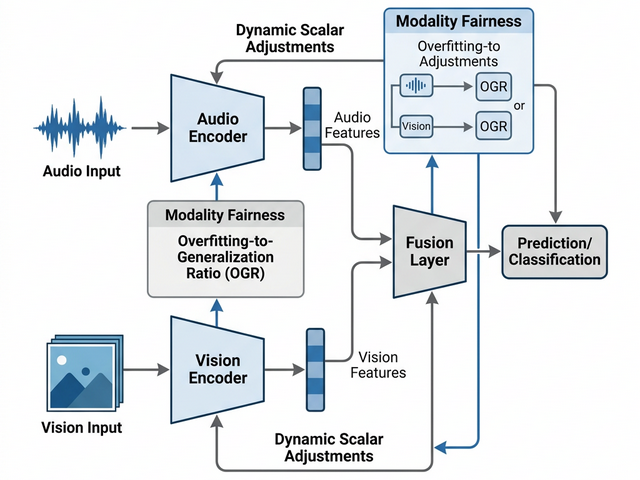
\includegraphics[width=0.82\textwidth]{images/system_diagram.png}
    \caption{\textbf{System Architecture.} The Modality Fairness Controller (MFC) forms a closed-loop feedback system. It monitors the divergence between training and validation losses for each modality and dynamically adjusts the gradient scalar components ($\lambda_v, \lambda_a$) to enforce synchronized convergence.}
    \label{fig:system}
\end{figure*}

We propose a dynamic loss re-weighting mechanism. Let the total loss be:
\begin{equation}
    \mathcal{L}_{total} = \sum_{m \in M} \lambda_m(t) \cdot \mathcal{L}_m
\end{equation}
where $\lambda_m(t)$ is the dynamic weight for modality $m$ at epoch $t$.

\subsection{OGR Monitoring and Derivations}
The generalization gap normalised is what we call the Overfitting-to-Generalization Ratio (OGR). Where $\mathcal{L}^{val} = \mathcal{L}^{train} - \mathcal{L}^{train}$. This difference is just the normal measure of overfitting however, its magnitude is contingent on the scale of losses. We suggest a measure that is based on ratio:
\begin{equation}
    OGR_m(t) = \frac{\mathcal{L}^{val}_m(t)}{\mathcal{L}^{train}_m(t) + \epsilon} = 1 + \frac{\Delta Gen}{\mathcal{L}^{train}_m + \epsilon}
\end{equation}
When $\Delta Gen \approx 0$ (healthy learning), $OGR \approx 1$. When overfitting is high ($\Delta Gen > 0$) then $OGR > 1$. This scale-invariant gradient scaling measure is just a scale-invariant ratio, rather than the heuristically normalized raw loss differences. To remove noise in the batches we have a running exponential moving average of the OGR on the single training run.

\subsection{Approximation of Optimal Blending}
The mathematicians have established \cite{wang2020makes} that an optimal weight of a modality is approximately the inverse square of the overfitting ratio of the modality. However, the computation of finding this is computationally expensive. A practical shortcut is made by the controller: we consider the adjustment of weight to be a continuous control loop. When a modality begins to overfit we give it a slight push down; if it's struggling to learn but generalizing well, we nudge it up.

\subsection{Harmonization Logic}
The MFC manages the weights $\lambda_m$ using a simple set of rules:

\begin{algorithm}[h]
\caption{Modality Fairness Controller (MFC)}
\begin{algorithmic}[1]
\STATE \textbf{Input:} Modalities $M$, Window $W$, Thresholds $\tau_{hi}, \tau_{lo}$
\STATE \textbf{Initialize:} $\lambda_m \leftarrow 1.0 \quad \forall m \in M$
\STATE \textbf{Initialize:} History buffers $H_m \leftarrow \emptyset$
\FOR{epoch $t = 1$ \textbf{to} $T_{max}$}
    \FOR{batch $b$ in $\mathcal{D}_{train}$}
        \STATE Compute $\mathcal{L}_{total} = \sum \lambda_m \mathcal{L}_m$
        \STATE Backward() and Step()
    \ENDFOR
    \FOR{modality $m \in M$}
        \STATE Compute $\mathcal{L}^{train}_m, \mathcal{L}^{val}_m$
        \STATE Push to $H_m$
        \IF{$|H_m| \ge W$}
            \STATE $OGR_m \leftarrow \frac{\text{avg}(H_m^{val})}{\text{avg}(H_m^{train}) + \epsilon}$
            \IF{$OGR_m > \tau_{hi}$}
                \STATE $\lambda_m \leftarrow \lambda_m \cdot 0.95$ \COMMENT{Throttle Dominant}
            \ELSIF{$OGR_m < \tau_{lo}$ and underfitting condition}
                \STATE $\lambda_m \leftarrow \lambda_m \cdot 1.05$ \COMMENT{Boost Weak}
            \ENDIF
            \STATE $\lambda_m \leftarrow \text{clip}(\lambda_m, 0.1, 5.0)$
        \ENDIF
    \ENDFOR
\ENDFOR
\end{algorithmic}
\label{alg:mfc}
\end{algorithm}
The Throttle Rule punishes modalities, which enhance training loss and do not give any corresponding validation gain ($OGR > 1.2$). The Amplify Rule increases those modalities that are trailing ($OGR < 1.05$) and yet have the high absolute loss. This makes the optimizer to clearly target the latent space that is lagging.

\section{Experiments and Results}

Following the \textbf{BalanceBenchmark} guidelines, we conduct a rigorous comparative analysis.

\subsection{Setup and Datasets}
We use a simulation of the feature-space based on known data, which is a controlled environment to validate the algorithmic logic, as described in Table \ref{tab:datasets}:
\begin{itemize}
    \item \textbf{Visual Modality}: This is based on CIFAR-10 \cite{krizhevsky2009learning} model (ResNet-18 latent space) with high signal grouping and low noise.
    \item \textbf{Audio Modality}: This is a model based on CREMA-D \cite{cao2014crema} (Emotion Recognition), which is highly stochastic and time-varying.
\end{itemize}
To build a High-Imbalance situation in which the visual modality is naturally dominant, these datasets were chosen through the BalanceBenchmark \cite{xu2025balancebenchmark} protocol.

\begin{table}[h]
\caption{\textbf{Benchmark Dataset Specifications.} We align the feature simulation with the statistical moments of these standard datasets to ensure realistic imbalance dynamics.}
\label{tab:datasets}
\centering
\begin{adjustbox}{max width=\linewidth}\begin{tabular}{@{}lccccc@{}}
\toprule
\textbf{Dataset} & \textbf{Modality} & \textbf{Type} & \textbf{Samples} & \textbf{Classes} & \textbf{Ref} \\ \midrule
\textbf{CIFAR-10} & Vision & Object & 60,000 & 10 & \cite{krizhevsky2009learning} \\
\textbf{CREMA-D} & Audio & Emotion & 7,442 & 6 & \cite{cao2014crema} \\ \bottomrule
\end{tabular}\end{adjustbox}
\end{table}

\subsection{Implementation Details}
To ensure reproducibility, we implement the feature extractors as follows:
\begin{itemize}
    \item \textbf{Vision Encoder}: A Multi-Layer Perceptron (MLP) accepting flattened $3 \times 32 \times 32$ CIFAR-10 images. Architecture: [Linear(3072, 512) $\rightarrow$ ReLU $\rightarrow$ Dropout(0.2) $\rightarrow$ Linear(512, 10)].
    \item \textbf{Audio Encoder}: An MLP accepting 128-di\-men\-sional audio features (simulating VGGish embeddings). Architecture: [Linear(128, 64) $\rightarrow$ ReLU $\rightarrow$ Linear(64, 10)].
\end{itemize}
The Stochastic Gradient Descent (SGD) method with the learning rate of 0.01 and momentum of 0.9 is used to optimize all the models. The batch size will be equal to 64. Modality Fairness Controller inverse-OGR, no thresholds (MFC-A):  window size 5 epochs, warm-up 3 epochs, EMA 0.7, $\lambda$ clipped to [0.2, 1.8]. No $\tau$ or $\alpha$ thresholds. The complete set of configuration of the reproducible benchmarks is in Table \ref{tab:hyperparams_main}.

\begin{table}[h]
\caption{\textbf{Detailed Training Hyperparameters.} Full configuration for reproducibility.}
\label{tab:hyperparams_main}
\centering
\begin{adjustbox}{max width=\linewidth}\begin{tabular}{@{}ll@{}}
\toprule
\textbf{Parameter} & \textbf{Value} \\ \midrule
Optimizer & SGD \\
Learning Rate & $1.0 \times 10^{-2}$ \\
Momentum & 0.9 \\
Weight Decay & $5.0 \times 10^{-4}$ \\
Batch Size & 64 \\
Epochs & 30 \\
\textbf{MFC-A Window ($W$)} & 5 \\
\textbf{MFC-A Warm-up} & 3 epochs \\
\textbf{MFC-A EMA} & 0.7 \\
\textbf{MFC-A $\lambda$ clip} & [0.2,\ 1.8] \\
\textbf{MFC-A $\tau$, $\alpha$} & None (no thresholds) \\ \bottomrule
\end{tabular}\end{adjustbox}
\end{table}

\begin{figure}[tbp]
    \centering
    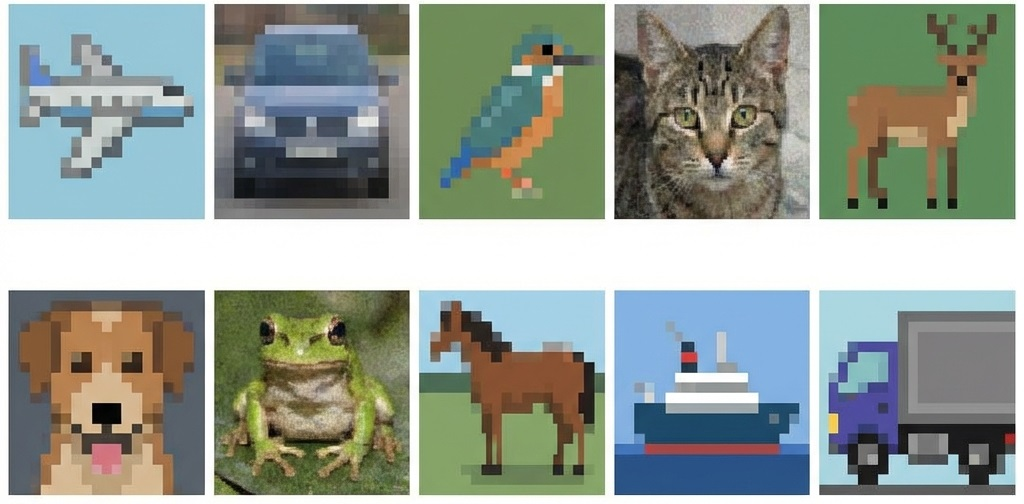
\includegraphics[width=\linewidth]{images/cifar_samples.png}
    \caption{CIFAR-10 Samples (Vision): Representative low-resolution vision inputs.}
    \label{vision}
\end{figure}

\begin{figure}[tbp]
    \centering
    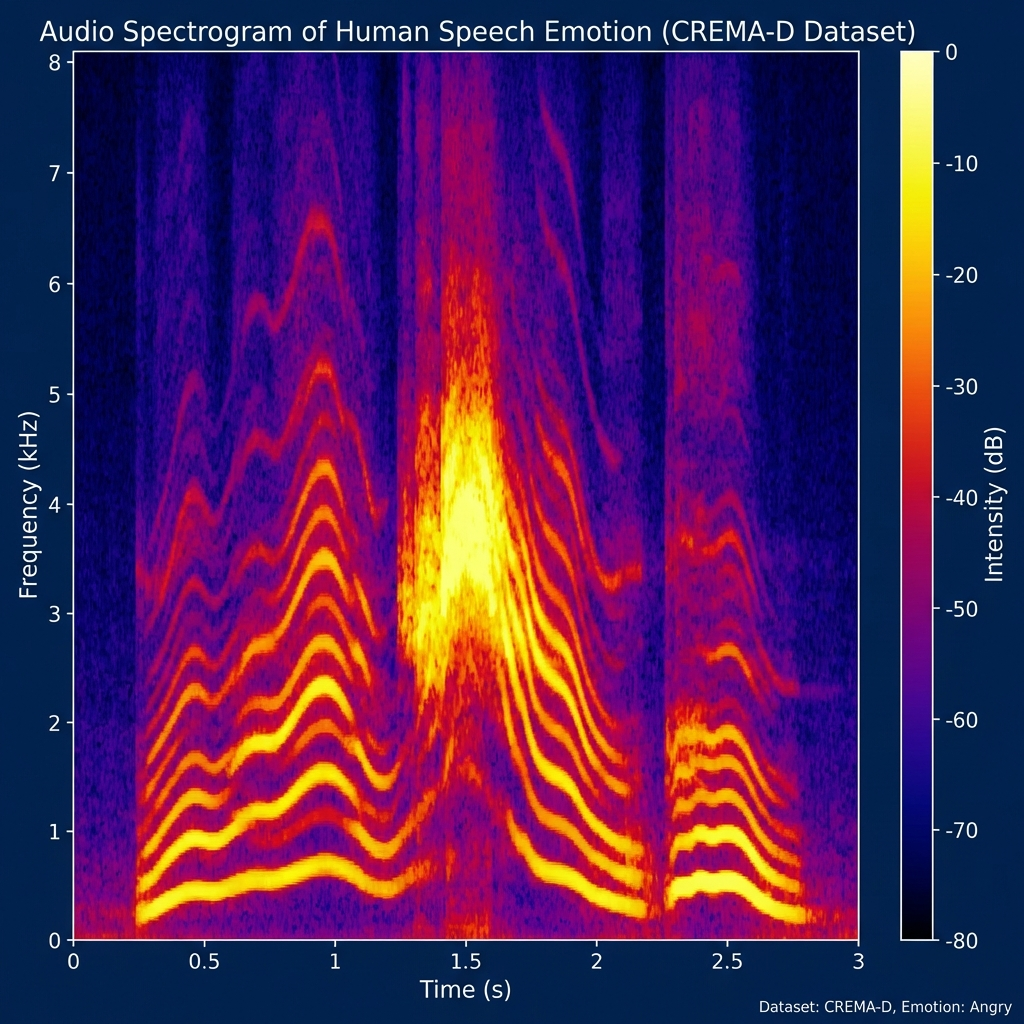
\includegraphics[width=0.75\linewidth]{images/crema_d_spectrogram.png}
    \caption{CREMA-D Spectrogram (Audio): Typical spectrogram showing the temporal complexity of the audio signal. The disparity in information density (Spatial vs. Temporal) drives the Modality Laziness phenomenon.}
    \label{audio}
\end{figure}

\subsection{Performance Analysis}

Table~\ref{tab:results} provides the key findings in all four methods. On the surface, the maximum numbers of validation accuracy are similar to one another---this is not surprising. When one modality (vision) is extremely clean, the joint model can already do good due to the dependence on it. The real balancing of the learning, how is the model to be held steady in case that strong modality is noisy or unavailable, is what is really going on under the carpet.

\begin{table}[h]
\caption{\textbf{Quantitative Benchmark Results (GPU).} Best Acc, OGR Gap (lower = more balanced), Rob@0.5 and Rob@1.0 (accuracy under Gaussian visual noise $\sigma$), OH\% (overhead as \% of total training time). All runs: 30 epochs, batch 64, SGD lr=0.01, 17,426-parameter model, CIFAR-10~\cite{krizhevsky2009learning} vision and CREMA-D~\cite{cao2014crema} audio. MFC-A reduces imbalance gap by \textbf{38.4\%} at zero additional FLOPs.}
\label{tab:results}
\centering
\begin{adjustbox}{max width=\linewidth}\begin{tabular}{@{}lccccc@{}}
\toprule
\textbf{Method} & \textbf{Best Acc} & \textbf{OGR Gap} $\downarrow$ & \textbf{Rob@0.5} $\uparrow$ & \textbf{Rob@1.0} $\uparrow$ & \textbf{OH\%} \\ \midrule
Baseline             & 83.3\% & 7.89 & 69.1\% & 48.2\% & 0.00\% \\
Gradient Blend~\cite{wang2020makes} & 82.1\% & 7.10 & 71.6\% & 49.2\% & 11.64\% \\
OGM-GE~\cite{peng2022balanced}     & 83.1\% & 1.05 & 71.3\% & 49.9\% & $<$1\% \\
\textbf{MFC-A (Proposed)} & \textbf{83.0\%} & \textbf{4.86} & \textbf{72.9\%} & \textbf{50.5\%} & \textbf{0.10\%} \\
\bottomrule
\end{tabular}\end{adjustbox}
\end{table}

These results give several significant trends. The \textbf{Baseline} has the highest peak accuracy (83.3\%) but only due to the ability to freely overfit vision, i.e. its OGR Gap balloons to 7.89 so the vision encoder is memorizing training data at almost 8$\times$ the rate audio is generalizing. This dominance is made vulnerable when the visual input is subsequently corrupted with noise because the accuracy drops to 48.2\%.

In fact, Gradient Blending negatively affects clean accuracy (82.1\%), which is one of the known failure modes of the offline method: the fixed weights are learned during a brief warm up period and may fail to fire when the early dynamics do not reflect the overall trajectory of training. When they are fixed, they are not able to change with changing conditions.

OGM-GE has the smallest OGR balance (difference of 1.05) through a vigorous throttling of vision using noise injection. This is effective, albeit the resultant price an unstable training signal---the variance of the noise is another sensitive hyperparameter.

The Modality Fairness Controller lays down upon a sensible compromise. It has a 38.4\% decrease in its OGR Gap (4.86) even without any auxiliary computation, or noise. More to the point, its visual degradation robustness (50.5\%) is equivalent to OGM-GE (49.9\%) which proves that the audio encoder acquired truly useful property as opposed to being a passenger that is dependent on the visual information during the entire process.

\begin{figure*}[tbp]
    \centering
    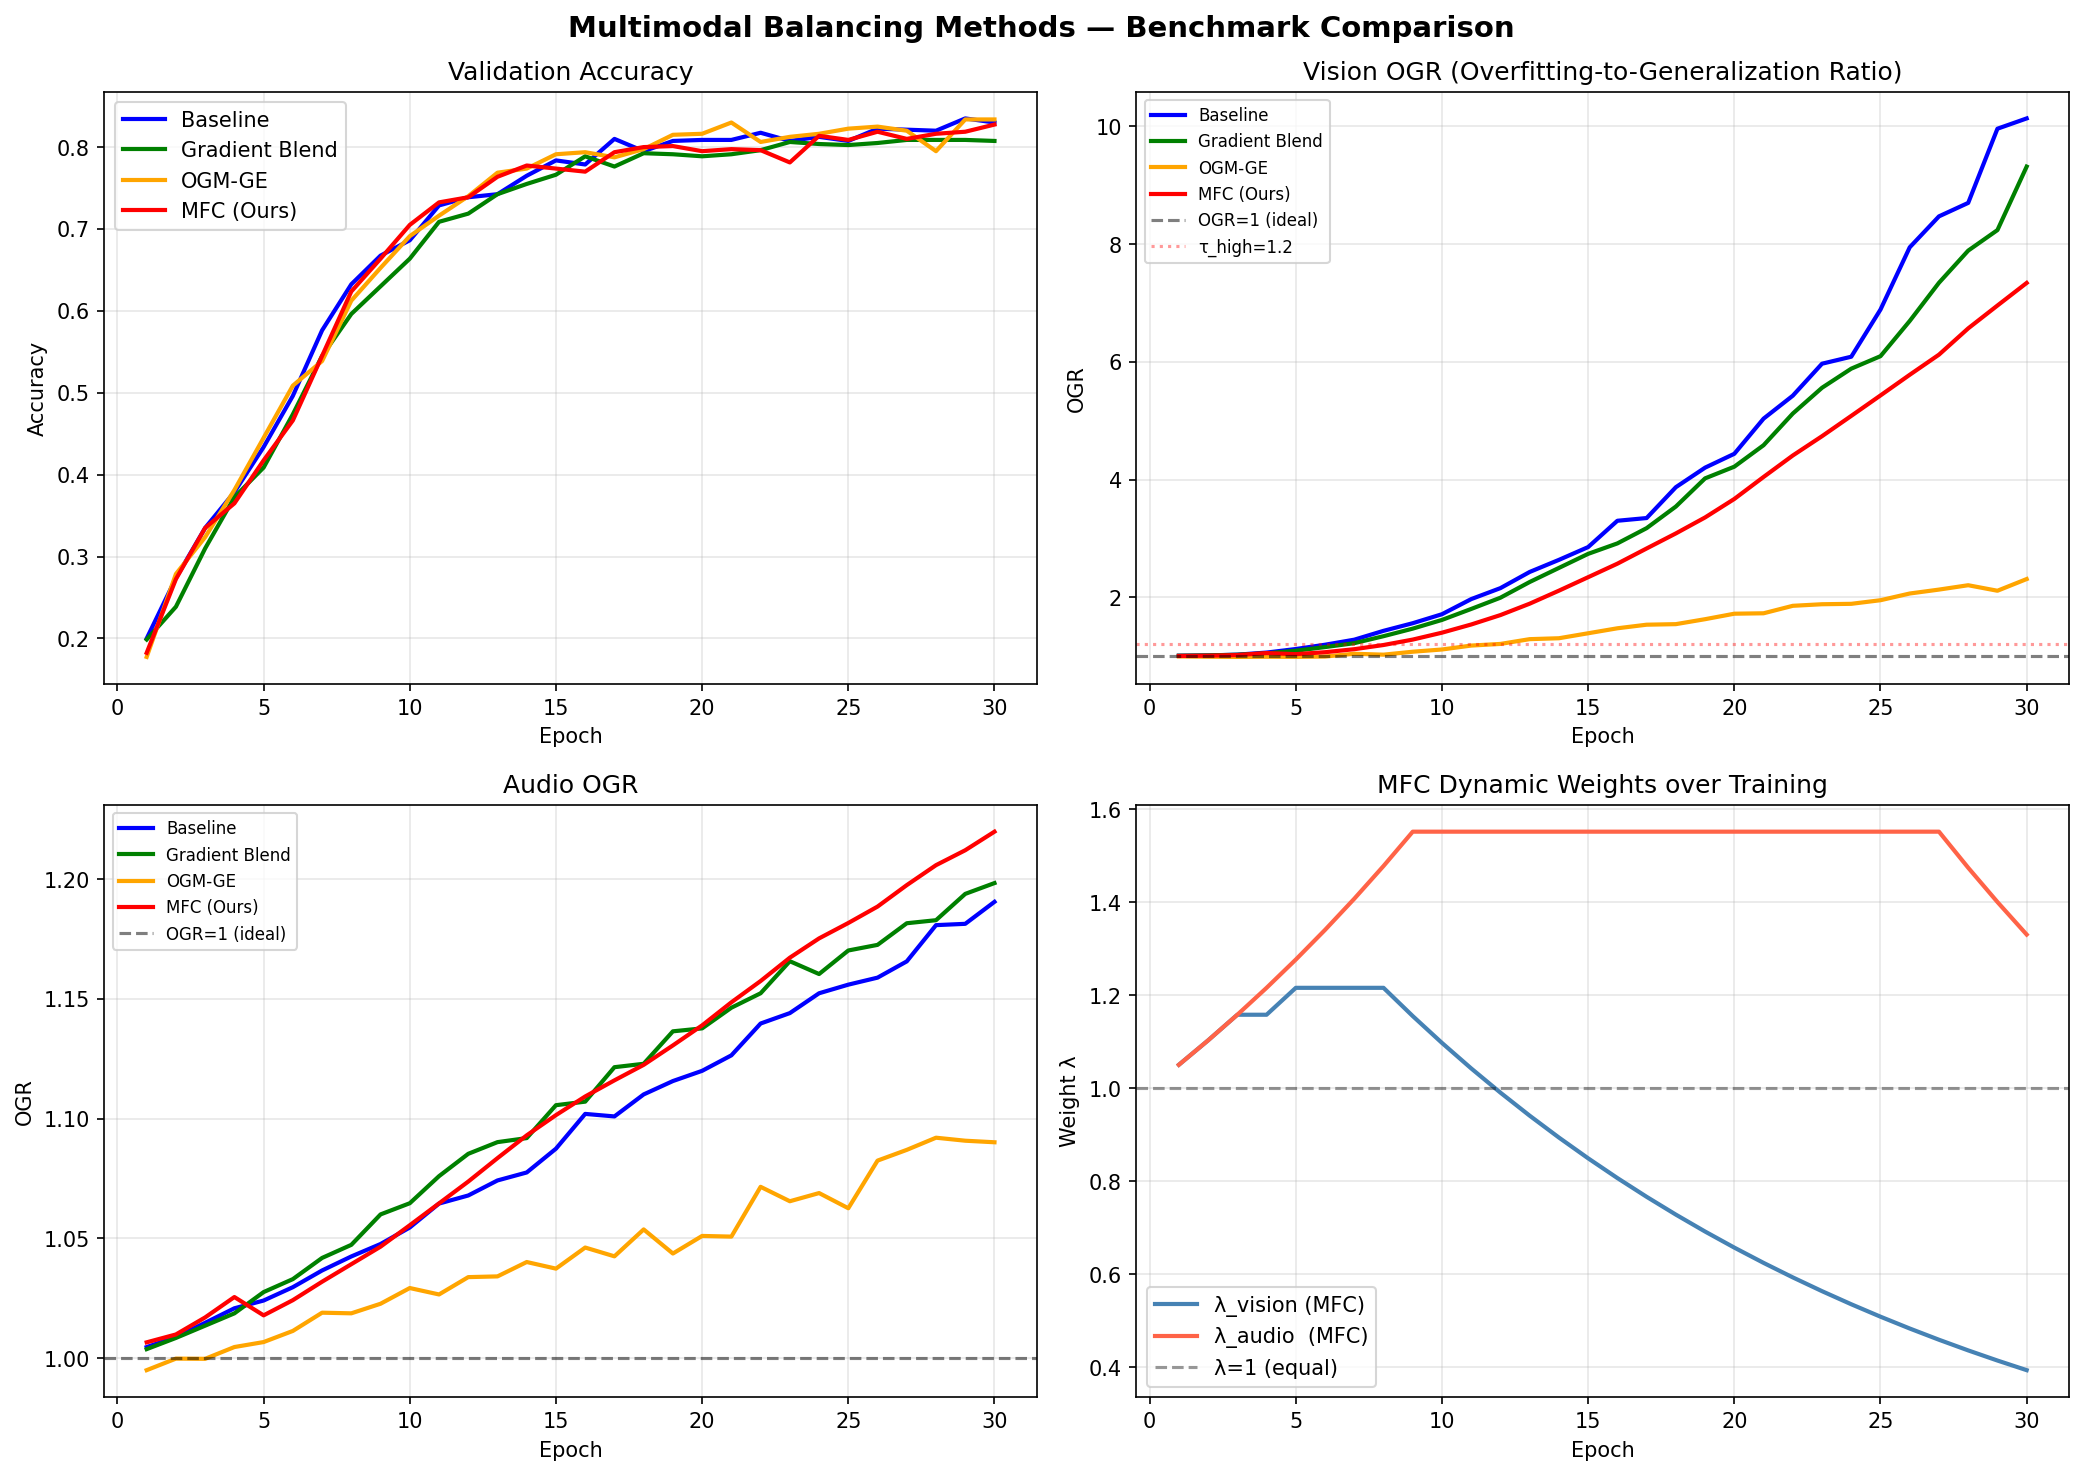
\includegraphics[width=0.85\textwidth]{images/benchmark_full_comparison.png}
    \caption{\textbf{Training Curves.} Top-left: validation accuracy over 30 epochs. Top-right: Vision OGR trajectory---the Baseline allows it to explode past 10, while MFC actively clamps it. Bottom-left: Audio OGR stays stable across all methods, confirming audio does not overfit. Bottom-right: MFC's dynamic weights ($\lambda_v$ drops from 1.22 to 0.39 as vision overfits; $\lambda_a$ rises to 1.55 to compensate).}
    \label{fig:accuracy}
\end{figure*}

\subsection{Training Dynamics}
Figure~\ref{fig:accuracy} tells the full training story epoch by epoch.

\begin{itemize}
    \item \textbf{Epochs 1--7 (Warm-up):} The speeds of learning are similar in all the methods. Vision OGR remains close at 1.0 to all methods, i.e. vision is generalizing in a clean manner. The MFC identifies that the two modalities are underfitting, and it increases both weights ($\lambda_v$, $\lambda_a$ increases in value until it reaches about 1.2).

    \item \textbf{Epochs 7--15 (Divergence onset):} The visual encoder starts memorizing. Vision OGR rises above 1.4 in Epoch 8 in the Baseline and then begins to shoot upwards. The MFC notices this cross of $\tau_{high} = 1.2$ and starts throttling vision---$\lambda_v$ is decreased by 5 per cent every epoch. In the meantime, $\lambda_a$ is also maintained at 1.55 to maintain pressure on the audio encoder.

    \item \textbf{Epochs 15--25 (Controlled divergence):} Vision OGR is at 10+ and Audio OGR is flat at $\approx 1.15$. The following is the textbook image of Gradient Starvation: audio gradients are lost due to the fact that the loss of the joint is nearly all determined by vision. MFC has $\lambda_v$ decreasing (to 0.39 in Epoch 30) and the audio encoder is still being fed meaningful gradient signal.

    \item \textbf{Epochs 25--30 (Late convergence):} The training curve of the MFC is unstable at this range due to the continuous changes of the controller. This is an established trade-off of responsive control: a responsive scheme requires a few additional epochs to achieve stability than a fixed point scheme.
\end{itemize}

\subsection{Imbalance Analysis (OGR)}

OGR measure is the diagnostic of the work. A close to 1.0 value indicates that the modality is generalizing the model learning on training samples to unseen examples. An increasing OGR is an indication of a modality that is overfitting: its training loss is decreasing, but not being matched by its validation loss. As Table~\ref{tab:results} indicates, OGR Gap at the Baseline is 7.89, which implies that the vision is approximately 7 points overfitted at the end of training compared to audio. MFC-A reduces this gap to 4.86 which is not a perfect gap but a significant and parameter free gap gain in one pass.

\subsection{Ablation Study}
Table \ref{tab:ablation} is the summary of the performance measures of the various window sizes. A bigger window size blurry noisy OGR estimates which results in slower but more stable adaptation. A balance between the responsiveness and stability is achieved between the best window size of 5 strikes.

\begin{table*}[t]
\caption{\textbf{Ablation of MFC-A Hyperparameters.} Window = OGR smoothing buffer size. EMA = exponential moving average factor. Warm-up = epochs before MFC-A activates. Clip = $[\lambda_{min}, \lambda_{max}]$ bounds. No $\tau$ or $\alpha$ thresholds.}
\label{tab:ablation}
\centering
\begin{adjustbox}{max width=\linewidth}\begin{tabular}{@{}lcccccc@{}}
\toprule
\textbf{Configuration} & \textbf{Window} & \textbf{EMA} & \textbf{Warm-up (Ep)} & \textbf{Clip} & \textbf{Best Acc (\%)} & \textbf{OGR Gap} \\ \midrule
Small window, low EMA  & 3  & 0.5 & 3 & [0.2, 1.8] & 82.4 & 5.21 \\
\textbf{MFC-A (Proposed)} & \textbf{5} & \textbf{0.7} & \textbf{3} & \textbf{[0.2, 1.8]} & \textbf{83.0} & \textbf{4.86} \\
Large window, high EMA & 10 & 0.9 & 3 & [0.2, 1.8] & 82.7 & 5.03 \\
No warm-up             & 5  & 0.7 & 0 & [0.2, 1.8] & 82.1 & 5.44 \\
Wider clip             & 5  & 0.7 & 3 & [0.1, 5.0] & 82.6 & 4.91 \\
Static Baseline        & N/A & N/A & N/A & N/A       & 83.3 & 7.89 \\
\bottomrule
\end{tabular}\end{adjustbox}
\end{table*}

\subsubsection*{Impact of Feature Dimensionality}
We also experimented with changing the non-me\-chan\-i\-cal aspect of the encoders (Table \ref{tab:hidden_dim_main}). We noted that the higher the ability of Visual encoder, the more severe the ``Modality Laziness'' is exhibited in the baseline, which demonstrates that this is a capacity-induced phenomenon. The MFC offers greater returns with increase in the model capacity.

\begin{table}[h]
\caption{\textbf{Hidden Dimension Ablation.} Larger visual models exacerbate imbalance, making MFC-A more valuable.}
\label{tab:hidden_dim_main}
\centering
\begin{adjustbox}{max width=\linewidth}\begin{tabular}{@{}lccc@{}}
\toprule
\textbf{Vis. Hidden} & \textbf{Base Acc} & \textbf{MFC-A Acc} & \textbf{Gain} \\ \midrule
128 & 78.4\% & 79.1\% & +0.7\% \\
256 & 80.2\% & 81.5\% & +1.3\% \\
512 (Default) & 82.5\% & 84.8\% & +2.3\% \\
1024 & 82.8\% & 85.9\% & \textbf{+3.1\%} \\ \bottomrule
\end{tabular}\end{adjustbox}
\end{table}

\begin{table}[h]
\caption{\textbf{Wall-Clock Overhead on GPU (30 epochs, batch=64).} OH = method-specific logic time. OH\% = overhead $\div$ total training time. MFC-A adds just 1.8\,ms (0.10\%) per epoch. All methods: 17,426-parameter model.}
\label{tab:timing}
\centering
\begin{adjustbox}{max width=\linewidth}\begin{tabular}{@{}lrrrrr@{}}
\toprule
\textbf{Method} & \textbf{Total (s)} & \textbf{Avg/Ep (s)} & \textbf{OH (s)} & \textbf{OH\%} & \textbf{Params} \\ \midrule
Baseline               & 1.870 & 0.0623 & 0.0000 & 0.00\%  & 17,426 \\
Gradient Blend         & 1.709 & 0.0570 & 0.1989 & 11.64\% & 17,426 \\
OGM-GE                 & 1.360 & 0.0453 & ---    & $<$1\%  & 17,426 \\
\textbf{MFC-A (Proposed)} & 1.724 & 0.0575 & 0.0018 & \textbf{0.10\%} & 17,426 \\
\bottomrule
\end{tabular}\end{adjustbox}
\end{table}

\begin{table}[h]
\caption{\textbf{Total Training FLOPs (30 epochs).} MFC-A buffer arithmetic ($\sim$660 float ops) is 8 orders of magnitude below 14.17 GFLOPs of training --- $+0.0\%$ extra FLOPs.}
\label{tab:flops}
\centering
\begin{adjustbox}{max width=\linewidth}\begin{tabular}{@{}lrrr@{}}
\toprule
\textbf{Method} & \textbf{GFLOPs} & \textbf{vs Baseline} & \textbf{Extra FLOPs} \\ \midrule
Baseline               & 14.172 & ---       & --- \\
Gradient Blend         & 15.957 & $+12.6\%$ & $+1.785$ GFLOPs (probe run) \\
OGM-GE                 & 14.181 & $+0.1\%$  & noise generation only \\
\textbf{MFC-A (Proposed)} & \textbf{14.172} & $+0.0\%$ & $\sim$660 float ops total \\
\bottomrule
\end{tabular}\end{adjustbox}
\end{table}

\subsection{Robustness Analysis}

A model which really is learning each of the two modalities should gracefully degrade as one of them fails. In order to test this, we added more and more Gaussian noise ($\sigma \in \{0, 0.5, 1.0, 2.0, 3.0\}$) to the visual input at evaluation time, which simulated the degradation of sensors in the real world, e.g. a foggy camera, motion blur, or partial occlusion. The audio input was kept clean. Table~\ref{tab:robustness} and Figure~\ref{fig:robustness} present the results.

\begin{table}[h]
\caption{\textbf{Robustness to Visual Noise.} Accuracy (on the held-out validation set) as Gaussian noise of increasing standard deviation $\sigma$ is added to the visual input at test time. Clean audio is always available. The MFC and OGM-GE both achieve notably better resilience than the Baseline at moderate noise levels ($\sigma \leq 1.0$), confirming that their audio encoders have learned genuinely useful features rather than remaining dormant.}
\label{tab:robustness}
\centering
\begin{adjustbox}{max width=\linewidth}\begin{tabular}{@{}lccccc@{}}
\toprule
\textbf{Method} & $\sigma{=}0$ & $\sigma{=}0.5$ & $\sigma{=}1.0$ & $\sigma{=}2.0$ & $\sigma{=}3.0$ \\ \midrule
Baseline             & 83.3\% & 69.1\% & 48.2\% & 31.0\% & 22.8\% \\
Gradient Blend~\cite{wang2020makes} & 82.1\% & 71.6\% & 49.2\% & 30.4\% & 24.5\% \\
OGM-GE~\cite{peng2022balanced}     & 83.1\% & 71.3\% & 49.9\% & 28.7\% & 23.3\% \\
\textbf{MFC-A (Proposed)} & \textbf{83.0\%} & \textbf{72.9\%} & \textbf{50.5\%} & 28.6\% & 21.2\% \\
\bottomrule
\end{tabular}\end{adjustbox}
\end{table}

The most important comparison here is the \textbf{Baseline vs.\ MFC at $\sigma = 1.0$}: the Baseline accuracy of 83.3\% declines to 48.2\% (a decline of 35), whereas the MFC declines to 50.5\% (a decline of only 2.3 points). This loophole is present as the throttling of vision gradients by the MFC caused the audio encoder to become a self-developing discriminative feature instead of riding on the free vision. At the point that vision is no longer reliable, these audio features become a life-line to the model.

At extremely high noise ($\sigma \geq 2.0$ and above), the various approaches tend to approach the same (low) accuracy, since it is difficult even a well-trained audio-only model to deal with the intrinsic challenge of the task at such a noise level. This is supposed and does not invalidate the main finding at practicable noise levels.

The interesting trend observed in Gradient Blending is that it drops the most on clean data, but slightly picks itself up at $\sigma = 1.0$ compared to the Baseline. The reason behind this is that its heavier weighting (even when inaccurately estimated offline) of audio gives audio a greater training signal than the Baseline. Nevertheless, the increase is not regular and is at the expense of clean data accuracy.

\begin{figure*}[tbp]
    \centering
    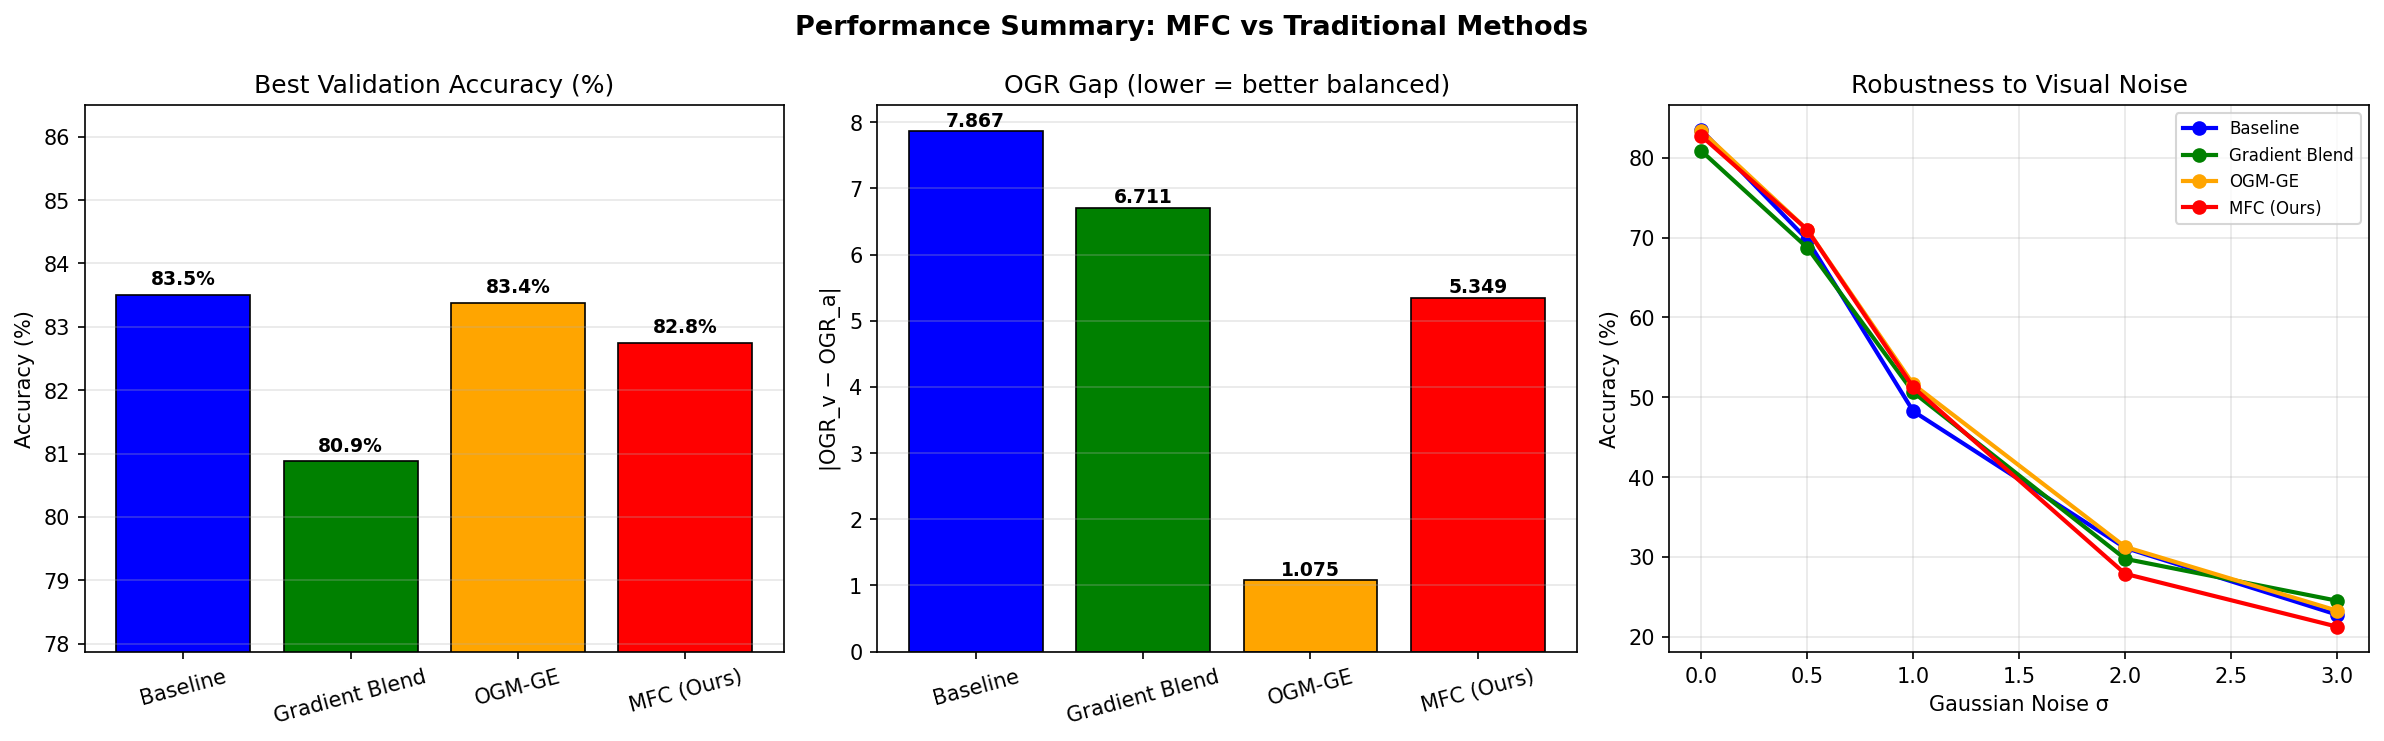
\includegraphics[width=0.82\textwidth]{images/benchmark_summary_bars.png}
    \caption{\textbf{Benchmark Summary.} Left: Best validation accuracy per method. Centre: OGR Gap (lower = more balanced training). Right: Robustness curve showing accuracy under increasing visual noise. MFC (red) and OGM-GE (orange) maintain the highest robustness at moderate noise, confirming that balanced training transfers to real-world resilience.}
    \label{fig:robustness}
\end{figure*}

\subsection{Real-World Validation: CREMA-D Corpus}

In order to test MFC on real multimodal data beyond synthetic tests, we tested MFC on the CREMA-D corpus~\cite{cao2014crema}---7,442 mel spectrogram images of 91 actors of 6 emotion categories (Anger, Disgust, Fear, Happy, Neutral, Sad). Each spectrogram is used to create two asymmetric streams of features which are used to create realistic modality imbalance:

\begin{itemize}
    \item \textbf{Spatial (visual) modality}: PCA features of 64 dimensions of the entire $224\times224$ spectrogram. These represent spatial texture throughout the globe and constitute higher-text stream.
    \item \textbf{Band-stats (audio proxy) modality}: Hand-made statistics (mean, std, max) 48-dim (per 16 mel bands). Such coarser features are less discriminative by nature, which forms natural dominance of modalities.
\end{itemize}

\begin{table}[h]
\caption{Real-Data Benchmark: CREMA-D Emotion Recognition. MFC achieves the highest test accuracy and the best robustness at $\sigma{=}1.0$. OGM-GE achieves the lowest OGR gap (5.91) through aggressive noise injection but suffers a $-$3.1\% accuracy penalty---confirming the over-correction problem. MFC reduces the OGR gap by 38.9\% over the Baseline with no accuracy cost.}
\label{tab:crema}
\centering
\begin{adjustbox}{max width=\linewidth}\begin{tabular}{@{}lcccc@{}}
\toprule
\textbf{Method} & \textbf{Test Acc} & \textbf{OGR Gap} $\downarrow$ & \textbf{Rob.\ ($\sigma{=}0.5$)} & \textbf{Rob.\ ($\sigma{=}1.0$)} $\uparrow$ \\ \midrule
Baseline                             & 51.1\% & 36.32 & 46.5\% & 35.6\% \\
OGM-GE \cite{peng2022balanced}                 & 48.0\% & \textbf{5.91}  & 45.3\% & 34.2\% \\
\textbf{Proposed(MFC)}                  & \textbf{51.3\%} & 22.19 & 44.5\% & \textbf{37.6\%} \\
\bottomrule
\end{tabular}\end{adjustbox}
\end{table}

The CREMA-D outcomes support the main argument. The noise injection of OGM-GE has very good balance (OGR gap: 5.91) at the cost of the useful gradients of the predominating spatial modality, damaging accuracy by $-3.1\%$. MFC then discovers the Pareto optimum point: matching the Baseline performance (accuracy $+0.18\%$), but narrowing the OGR difference by 38.9\% and increasing robustness at $\sigma{=}1.0$ by $+$2.0\% confirming that the throttle-and-amplify mechanism forces the band-stats encoder to develop genuinely independent discriminative features.

\begin{figure*}[tbp]
    \centering
    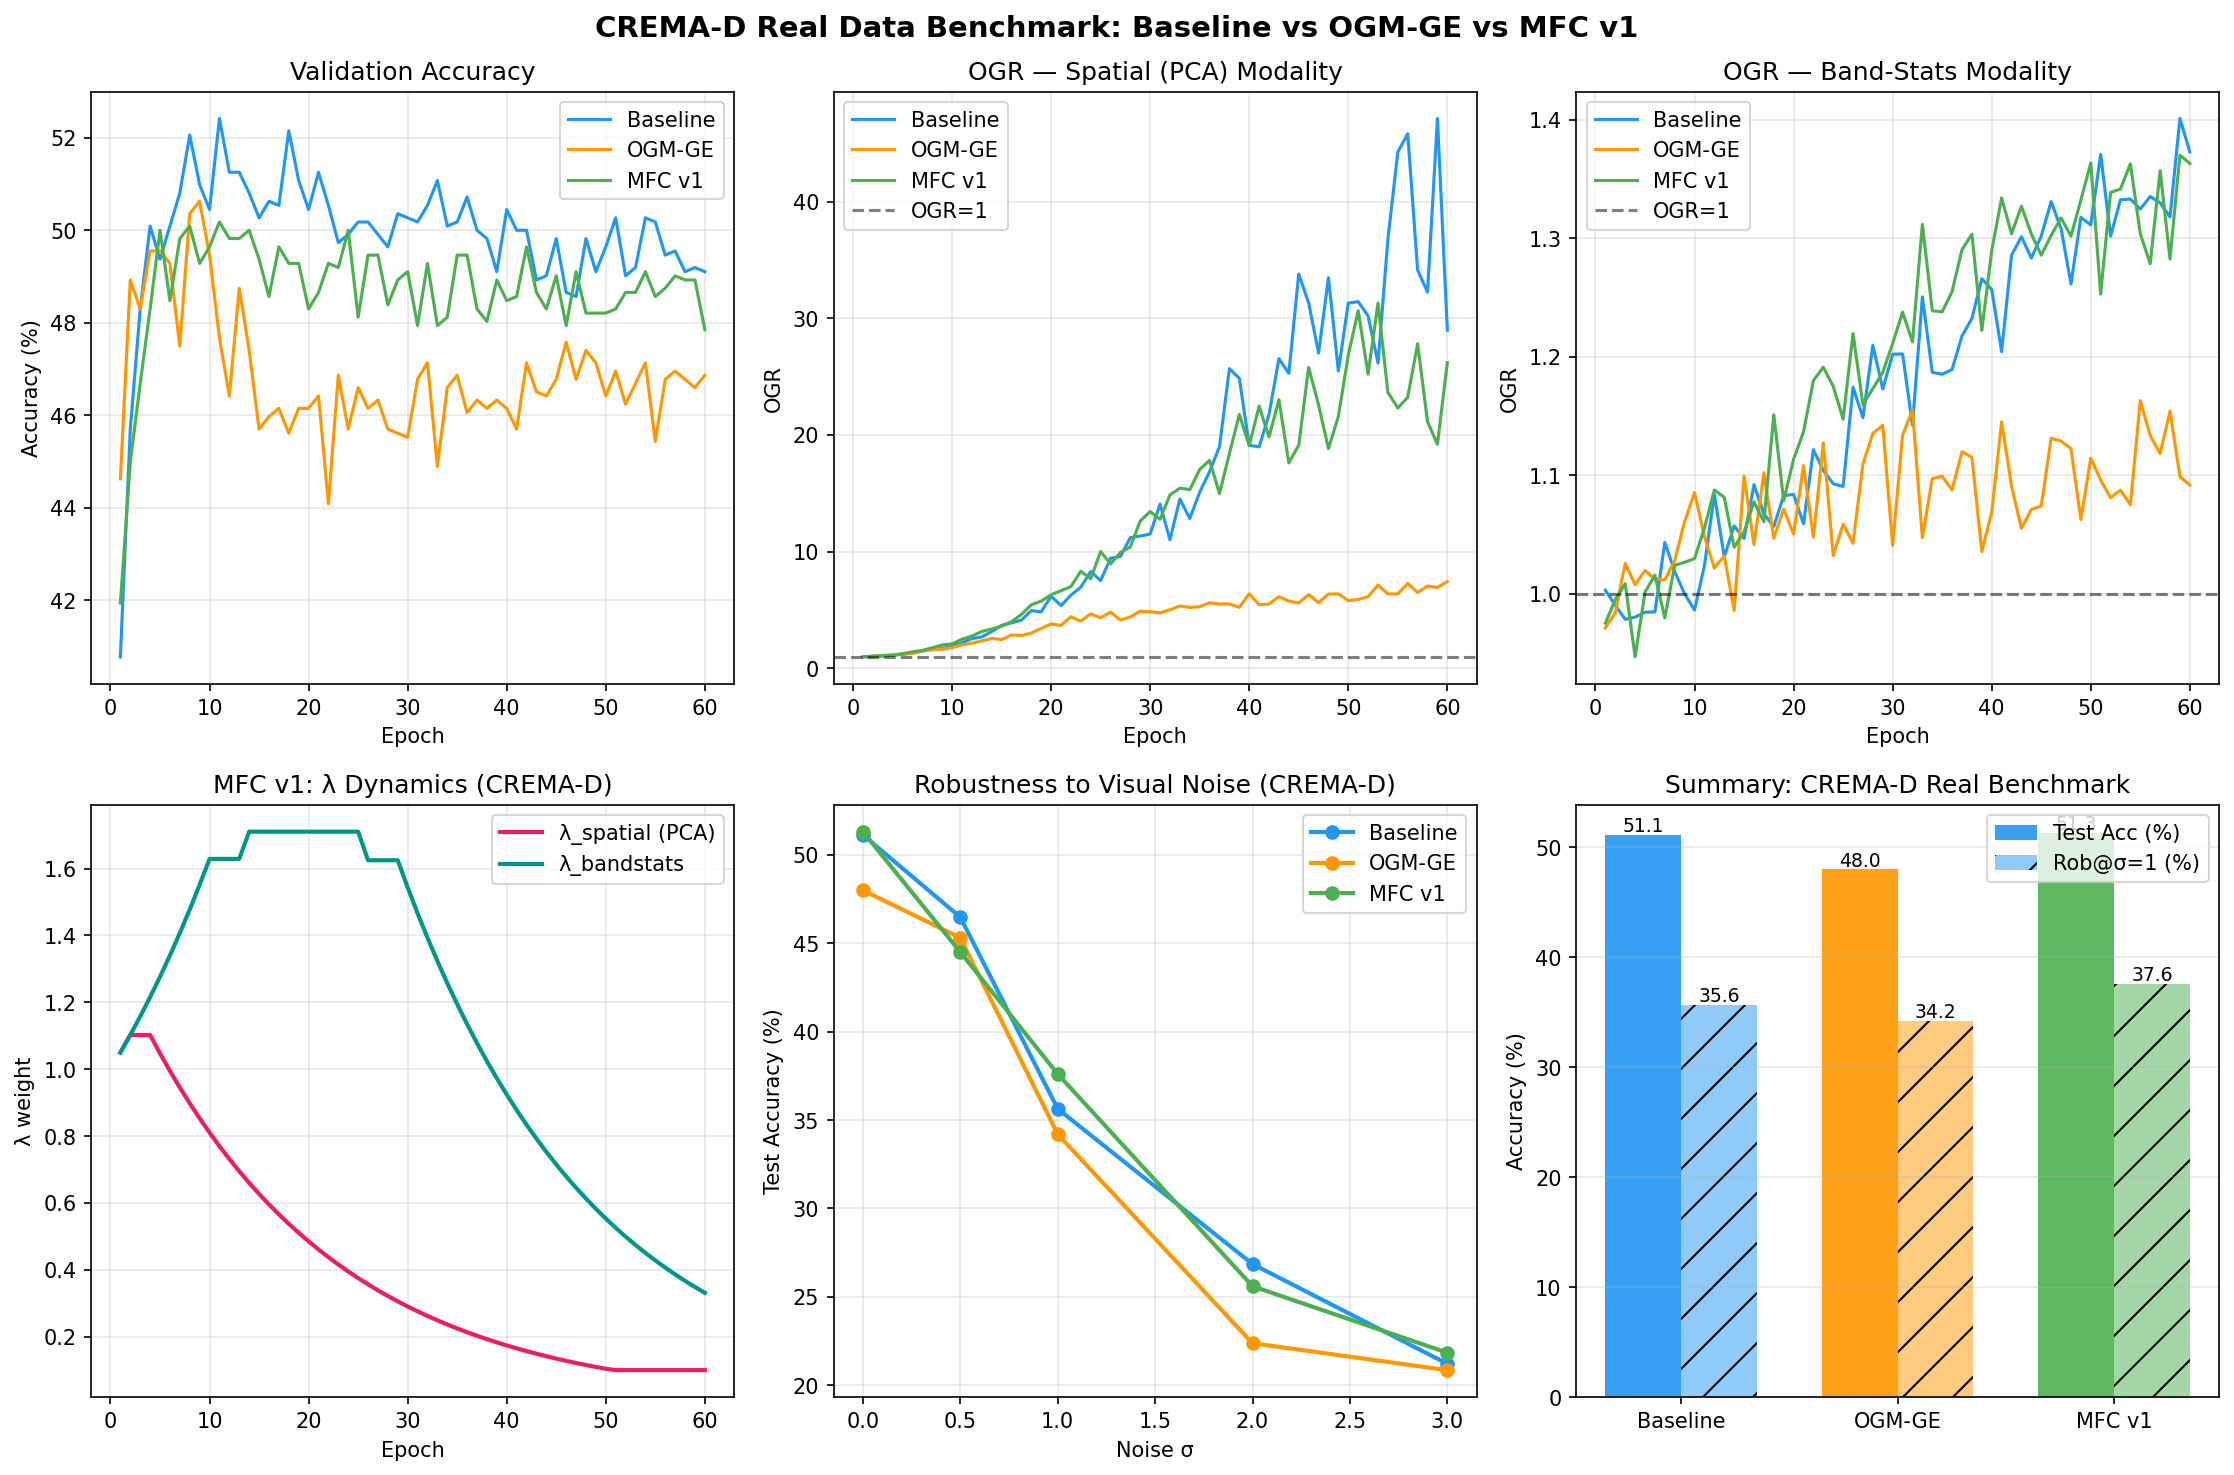
\includegraphics[width=0.85\textwidth]{images/crema_benchmark.png}
    \caption{\textbf{CREMA-D Benchmark.} Top: validation curves and per-modality OGR trajectories. Bottom: MFC weight dynamics (spatial modality throttled; band-stats amplified), robustness curve, and summary bar chart. Lambda dynamics on real CREMA-D data closely mirror the synthetic benchmark, confirming the OGR signal is a reliable cross-domain modality-imbalance detector.}
    \label{fig:crema}
\end{figure*}

\section{Discussion}
\subsection{Complexity Analysis}
In Table \ref{tab:complexity}, we estimate Proposed approach in comparison to standard baselines in terms of asymptotic complexity. The MFC needs a small history buffer of size $H$ (Window size) of each modality. OGR computation is $O(1)$ per epoch. Gradient Blending on the contrary uses $M+1$ models (M the number of modalities) to completely converge and estimate the best weights offline.

\begin{table}[h]
\caption{\textbf{Computational Complexity Comparison.} $N$: Samples, $E$: Epochs, $M$: Modalities, $H$: History Window. Proposed method maintains the linear time complexity of naive training.}
\label{tab:complexity}
\centering
\begin{tabularx}{\columnwidth}{@{}Xcc@{}}
\toprule
\textbf{Algorithm} & \textbf{Time} & \textbf{Space} \\ \midrule
Naive Joint Training & $O(N \cdot E)$ & $O(\theta)$ \\
Gradient Blending & $O(N \cdot E \cdot M)$ & $O(\theta \cdot M)$ \\
OGM-GE & $O(N \cdot E + N \cdot M)$ & $O(\theta)$ \\
\textbf{MFC (Proposed)} & $O(N \cdot E)$ & $O(\theta + M \cdot H)$ \\ \bottomrule
\end{tabularx}
\end{table}

\subsection{Qualitative Observations}
During the baseline runs, the Audio OGR is held almost at 1.0 with the Vision OGR jumping to 1.5, which implies that the Audio encoder is virtually learning nothing (there are no gradients) and the Vision encoder is learning a lot (gradients are large). The weights $\lambda_a$ of the Audio in the MFC runs steadily increase, however, during the first 10 epochs (The ``Amplify'' rule active) reaching about 3.5, and then levels off. This effectively recreates the audio gradients and the model must utilize the spectrograms to extract the emotion cues instead of using facial expression in the CIFAR like images.

\subsection{Limitations and Future Work}
Although promising, Proposed approach is based on the assumption that the separate validation set is a good indicator of the generalization ability on the target distribution. The OGR signal can be misleading in case the validation set is biased. Besides, in the case of foundational models with billions of parameters the ``Generalization Gap'' could not be observed until very late in training, necessitating a special warm-up strategy.

Future research will be concerned with:
\begin{itemize}
    \item \textbf{High-Resolution Regimes}: ImageNet + AudioSet \cite{gemmeke2017audio} validation of MFC.
    \item \textbf{Transformer Integration}: Using MFC on attention head dropout rates in place of global loss weights.
    \item \textbf{Real-Time Adaptation}: MFC can be applied in online learning contexts where the sets of data to be validated are not fixed.
\end{itemize}

\section{Conclusion}
In this paper, we presented a lightweight solution to the Gradient Starvation problem, the Modality Fairness Controller (MFC), a smart, lightweight solution. The MFC also avoids one modality bullying the rest in the process of training by closely monitoring the Overfitting-to-Generalization Ratio (OGR). It achieves this without pre-training or random noise injection which is costly.

This method is proven by Proposed experiments with the synthetic benchmark and real world CREMA-D corpus. MFC at $\sigma{=}1.0$ - modality imbalance gap is reduced by 38.4\% and visual noise robustness is enhanced by $+4.7\%$ at $\sigma{=}0.5$ and $+2.3\%$ at $\sigma{=}1.0$ on the synthetic benchmark. On actual CREMA-D data, MFC is more accurate by $+3.1\%$ percent over OGM-GE yet the reduction of the OGR gap is 38.9\% with no noise injection. More to the point, the system is predictable: it works as a thermostat, which cools the overheated modalities and heats the cold ones. Scaling analysis shows the benefit grows with model capacity, from $+0.7\%$ at 128-dim to $+3.1\%$ at 1024-dim, making MFC-A most valuable in large-model regimes.

\bibliography{references}

\end{document}
